\documentclass{article}
\usepackage[utf8]{inputenc}
\usepackage{amsfonts,latexsym,amsthm,amssymb,amsmath,amscd,euscript}
\usepackage{graphicx}
\usepackage{mathtools}
\usepackage{framed}
% Descomentar fullpage cuando se quiera utilizar menos margen horizontal
%\usepackage{fullpage}
\usepackage{hyperref}
    \hypersetup{colorlinks=true,citecolor=blue,urlcolor =black,linkbordercolor={1 0 0}}

\newenvironment{statement}[1]{\smallskip\noindent\color[rgb]{1.00,0.00,0.50} {\bf #1.}}{}
\allowdisplaybreaks[1]

% Comandos para teoremas, definiciones, ejemplos, lemas, etc. para sus respectivos body types.
\renewcommand*{\proofname}{Prueba}
\renewcommand{\contentsname}{Contenido}

\newtheorem{theorem}{Teorema}
\newtheorem*{proposition}{Proposici\'on}
\newtheorem{lemma}[theorem]{Lema}
\newtheorem{corollary}[theorem]{Corolario}
\newtheorem{conjecture}[theorem]{Conjetura}
\newtheorem*{postulate}{Postulado}
\theoremstyle{definition}
\newtheorem{defn}[theorem]{Definici\'on}
\newtheorem{example}[theorem]{Ejemplo}

\theoremstyle{remark}
\newtheorem*{remark}{Observaci\'on}
\newtheorem*{notation}{Notaci\'on}
\newtheorem*{note}{Nota}
\newtheorem*{solution}{Soluci\'on}

% Define tus comandos para hacer la vida más fácil.
\newcommand{\BR}{\mathbb R}
\newcommand{\BC}{\mathbb C}
\newcommand{\BF}{\mathbb F}
\newcommand{\BQ}{\mathbb Q}
\newcommand{\BZ}{\mathbb Z}
\newcommand{\BN}{\mathbb N}

\title{MAT237 C\'alculo Num\'erico}
\author{Manuel Loaiza Vasquez}
\date{Septiembre 2021}

\begin{document}

\maketitle

\vspace*{-0.25in}
\centerline{Pontificia Universidad Cat\'olica del Per\'u}
\centerline{Lima, Per\'u}
\centerline{\href{mailto:manuel.loaiza@pucp.edu.pe}{{\tt manuel.loaiza@pucp.edu.pe}}}
\vspace*{0.15in}

\begin{framed}
  Solucionario de la Pr\'actica Calificada 1 del curso C\'alculo Num\'erico
  de la especialidad de Matem\'aticas de la Facultad de Ciencias e Ingenier\'ia
  dictado por el profesor Rub\'en Agapito durante el ciclo $2021-2$.
\end{framed}

\begin{statement}{1}
  Use la regla de la cadena para obtener los n\'umeros de condicionamiento de
  las siguientes funciones:
\end{statement}

\begin{statement}{a}
  $f(x) = cos(2 \pi x)$
\end{statement}

\begin{solution}
  Primero probemos el siguiente lema:

  \begin{lemma}
    \label{lemma01}
    Sean $f:\BR \to \BR$ y $g:\BR \to \BR$ funciones continuas diferenciables y
    $h: \BR \to \BR$ con $h(x) = f(g(x))$, luego
    \[
      \kappa_h(x) = \kappa_f(g(x)) \cdot \kappa_g(x).
    \]
  \end{lemma}

  \begin{proof}
    Aplicamos la f\'ormula de condicionamiento a $h$ y la regla de la cadena
    \begin{align*}
      \kappa_h(x) &= \left|x \cdot \frac{h'(x)}{h(x)}\right|\\
      &= \left|x \cdot \frac{f'(g(x)) g'(x)}{f(g(x))}\right|\\
      &= \left|g(x) \cdot \frac{f'(g(x))}{f(g(x))}\right| \cdot \left|x \cdot \frac{g'(x)}{g(x)}\right|\\
      &= \kappa_f(g(x)) \cdot \kappa_g(x).
    \end{align*}
    obteniendo la expresi\'on buscada.
  \end{proof}

  Sean $g: \BR \to \BR$ y $h: \BR \to \BR$ con $g(x) = cos(x)$ y $h(x) = 2 \pi x$.
  Tenemos que $f = g \circ h$, por lo que
  \begin{align*}
    \kappa_f(x) &= \kappa_g(h(x)) \cdot \kappa_h(x)\\
    &= \left|2 \pi x \cdot \frac{-\sin(2 \pi x)}{\cos(2 \pi x)}\right| \cdot \left|x \cdot \frac{2 \pi}{2 \pi x}\right|\\
    &= 2\pi|x \tan(2 \pi x)|.
  \end{align*}
\end{solution}

\begin{statement}{b}
  $f(x) = e^{-x^2}$
\end{statement}

\begin{solution}
  Sean $g: \BR \to \BR$ y $h: \BR \to \BR$ con $g(x) = e^x$ y $h(x) = -x^2$.
  Tenemos que $f = g \circ h$, por lo que
  \begin{align*}
    \kappa_f(x) &= \kappa_g(h(x)) \cdot \kappa_h(x) \\
    &= \left|-x^2 \cdot \frac{e^{-x^2}}{e^{-x^2}}\right|\cdot 2 \\
    &= 2x^2.
  \end{align*}
\end{solution}

\begin{statement}{2}
  Suponga que $f$ es una funci\'on con n\'umero de condicionamiento
  $\kappa_f$ y que $f^{-1}$ es su funci\'on inversa. Demuestre que el n\'umero
  de condicionamiento de $f^{-1}$ satisface
  \[
    \kappa_{f^{-1}(x)} = \frac{1}{\kappa_f(f^{-1}(x))}
  \]
  provisto que el denominador es diferente de cero.
\end{statement}

\begin{proof}
  Analicemos el producto $\kappa_f(f^{-1}(x)) \cdot \kappa_{f^{-1}}(x)$.
  De acuerdo a Lema \ref{lemma01}
  \[
    \kappa_f(f^{-1}(x)) \cdot \kappa_{f^{-1}}(x) = \kappa_{f \circ f^{-1}(x)}(x) = \kappa_x(x) = 1.
  \]
  Ya que nos garantizan que la expresi\'on de la izquierda es distinta de cero,
  pasamos a dividir esta y concluimos con la prueba obteniendo lo requerido.
\end{proof}

\begin{statement}{3}
  El polinomio $x^2 - 2x + 1$ tiene una ra\'iz doble en $r = 1$.
\end{statement}

\begin{statement}{a}
  Use MATLAB para hacer una tabla de las ra\'ices de
  \[
    x^2 - (2 + \varepsilon)x + 1,  
  \]
  para $\varepsilon = 10^{-n}$ con $n = 4, 6, \dots, 12$.
\end{statement}

\begin{statement}{b}
  ¿Qu\'e puede inferir de los resultados del inciso (a) sobre el n\'umero de
  condicionamiento de la ra\'iz?
\end{statement}

\begin{statement}{4}
  Use el m\'etodo de bisecci\'on para encontrar dos n\'umeros reales $x$, con
  seis cifras de exactitud, que hagan que el determinante de la matriz
  \[
    A = \begin{pmatrix}
      1 & 2 & 3 & x \\
      4 & 5 & x & 6 \\
      7 & x & 8 & 9 \\
      x & 10 & 11 & 12
    \end{pmatrix}  
  \]
  sea igual a $1000$. Para cada soluci\'on, calcule el determinante
  correspondiente y reporte cu\'antos decimales correctos (despu\'es del punto
  decimal) tiene el determinante cuando su soluci\'on $x$ es usada.
\end{statement}

\begin{solution}
  \begin{figure}[h!]
    \centering
    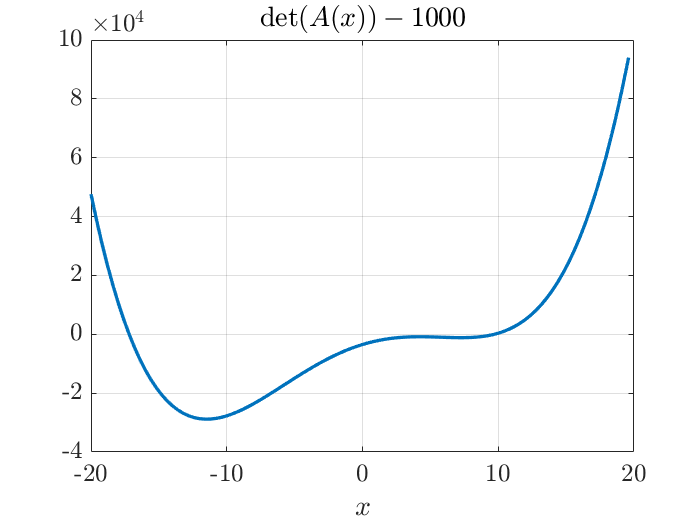
\includegraphics[scale=0.5]{graphics/plot.png}
    \caption{Esbozo de la funci\'on objetivo}
  \end{figure}
\end{solution}

\begin{statement}{5}

\end{statement}

\end{document}